\documentclass[11pt,letterpaper,final]{report}
\usepackage[utf8]{inputenc}
\usepackage[francais]{babel}
\usepackage[T1]{fontenc}
\usepackage{amsmath}
\usepackage{amsfonts}
\usepackage{amssymb}
\usepackage{graphicx}
\usepackage{lmodern}
\usepackage[left=2.54cm,right=2.54cm,top=2.54cm,bottom=2.54cm]{geometry}
\begin{document}
\chapter{Cross validation entre les différentes plateformes de simulations}
Dans ce chapitre, les simulateurs seront comparés selon les paramètres des simulations critiques (courant dans les électroaimants, tension aux bornes des électroaimants, courant d'entrée, tension du bus CC, etc.). Les différences seront analysées selon les sous-modèles implantés, qui seront détaillés plus loin dans cet ouvrage. Les sous-modèles se séparent en plusieurs catégories, soit les simulations représentant l'AFE, celles représentant le convertisseur CC-CC et celles représentant un montage avec un AFE et un convertisseur CC-CC. Il est à noté que les temps de simulation qui seront employés pour fins d'analyse sont de 50$\mu$s, de 5$\mu$s et de 1$\mu s$. 
\section{Pont DCP/DCN: Validation PSIM/SPS}
\subsection{Hacheur 4 quadrants}
Le hacheur 4 quadrants, à proprement parlé, est constitué de 4 interrupteurs IGBT commandés au moyen d'une régulation MLI. La figure INSÉRER UNE FIGURE MONTRANT LE HACHEUR 4 QUADRANTS présente une représentation schématique d'un tel convertisseur. Ce type de montage est un montage de base utilisé afin de valider le concept de fonctionnement d'un convertisseur CC-CC et afin d'établir la méthodologie de comparaison des simulations.
\subsubsection{Vérification pour un pas de calcul de 50$\mu$s}
Cette section présente les courbes d'intérêt pour un pas de calcul discret de 50$\mu$s. La figure \ref{comp_PSIM_SPS} présente le courant à la charge sur PSIM et SPS pour un pas de clacul de 50 $\mu$s. Sur cette figure, on remarque que les différences entre les deux courants avoisinent les 25A. Aussi, la courbe de PSIM est décalée d'environ 250$\mu$s vers la droite par rapport à celle de SPS. DÉCRIRE LES DIFFÉRENCES ICI. Il faut inclure les justifications etc. Il faut identifier chacune des courbes, et expliquer ce que l'on doit observer.

\begin{figure}[htb]
\centering
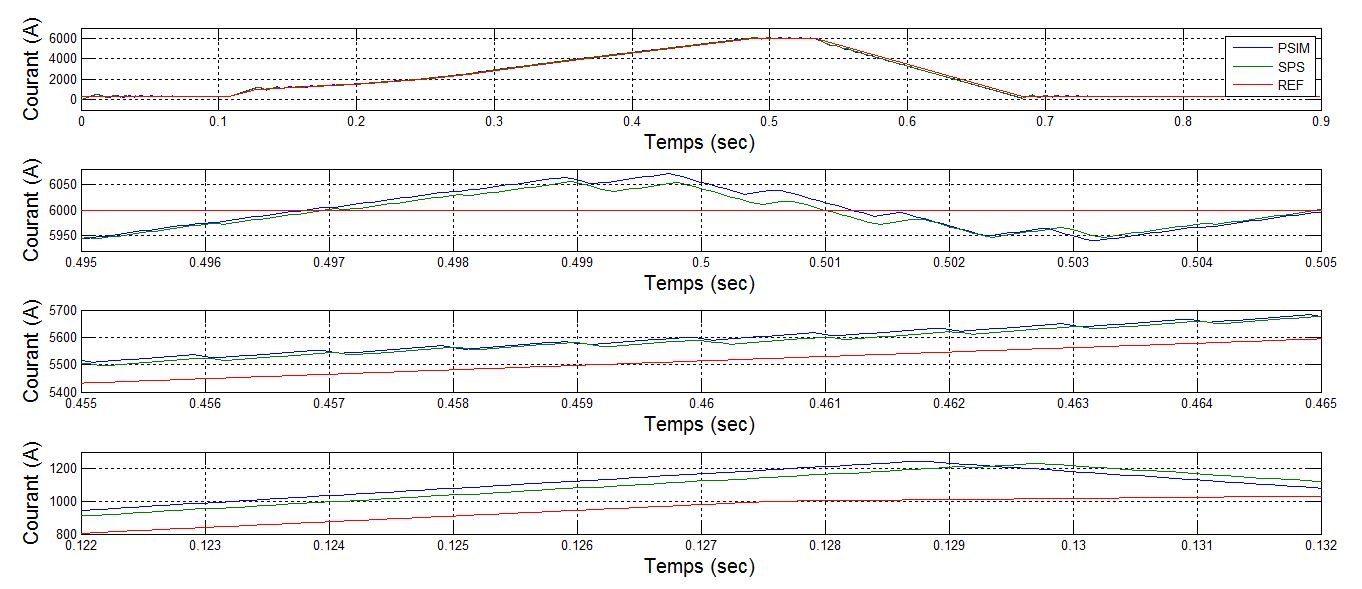
\includegraphics[scale=0.5]{Fig/Hacheur4Quadrants/HacheurCourantCharge50u.jpg}
\caption{Courant à la charge sur PSIM et SPS pour un pas de calcul de 50$\mu$s}.
\label{comp_PSIM_SPS}
\end{figure}


\begin{figure}[htb]
\centering
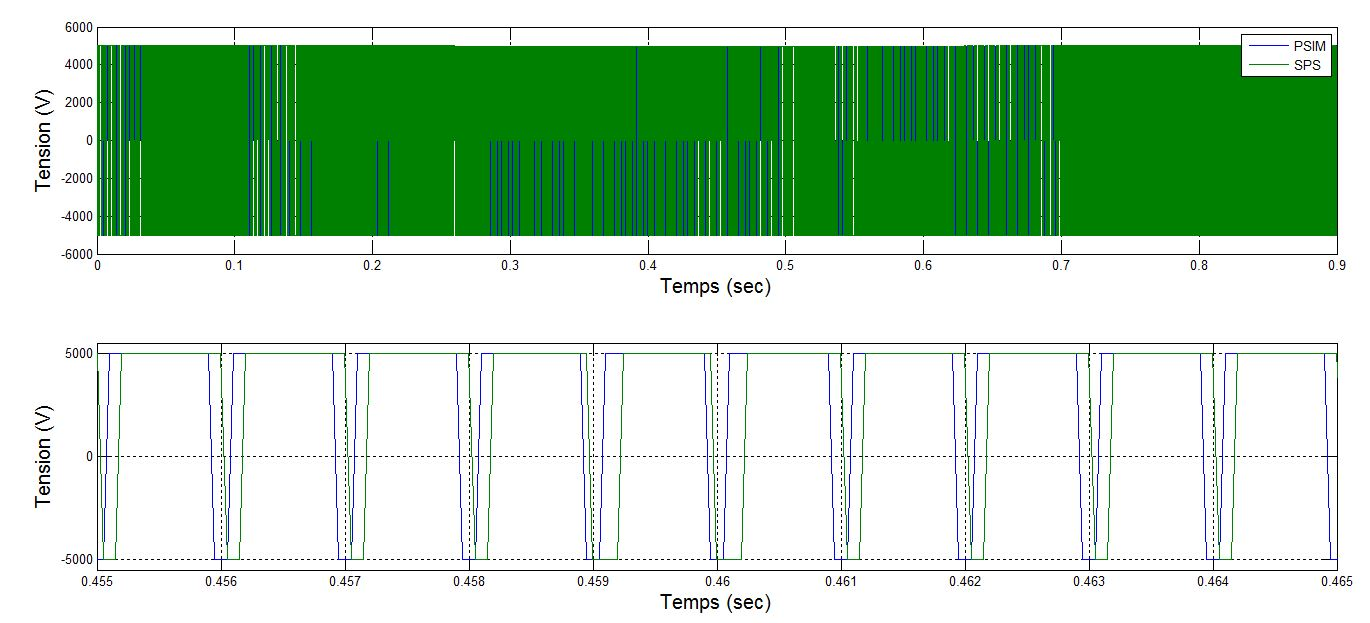
\includegraphics[scale=0.5]{Fig/Hacheur4Quadrants/HacheurTensionCharge50u.jpg}
\caption{Tension aux bornes de la charge sur PSIM et SPS pour un pas de calcul de 50$\mu$s}
\label{err_cou}
\end{figure}


\begin{figure}[htb]
\centering
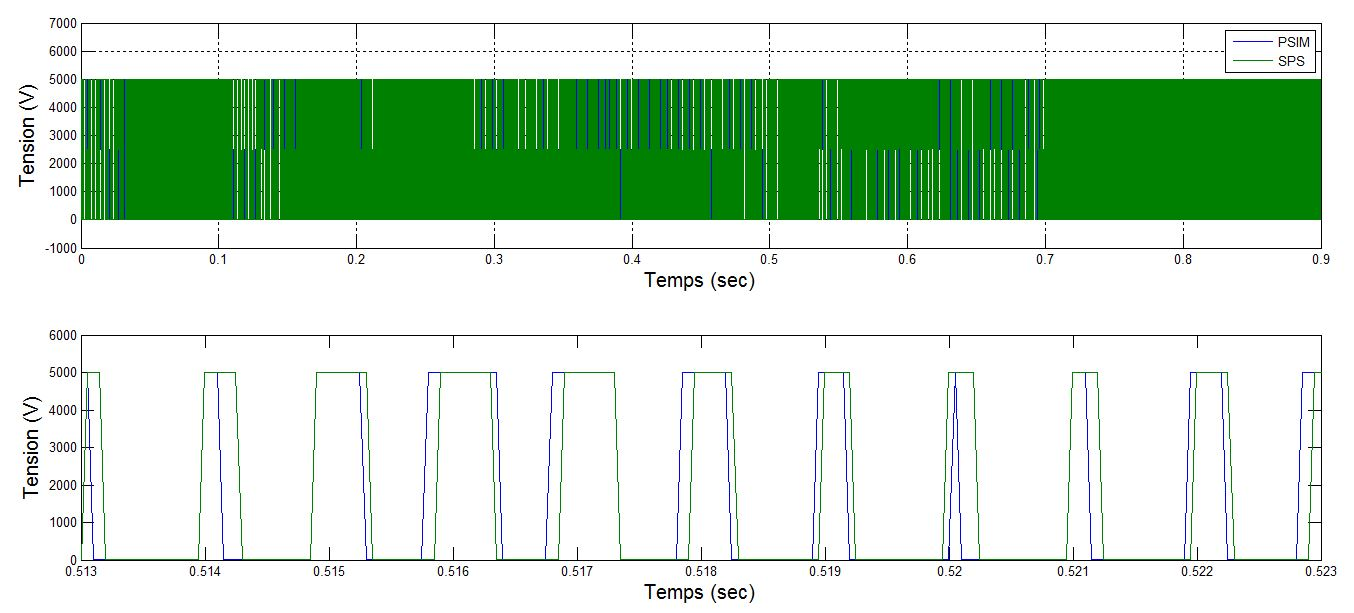
\includegraphics[scale=0.5]{Fig/Hacheur4Quadrants/HacheurTensionIGBT50u.jpg}
\caption{Tension aux bornes d'un IGBT sur PSIM et SPS pour un pas de calcul de 50$\mu$s}
\label{hc_IG_ten_50}
\end{figure}

\clearpage
\subsubsection{Vérification pour un pas de calcul de 5$\mu$s}
Cette section présente les courbes d'intérêt pour un pas de calcul discret de 5$\mu$s.DÉCRIRE LES DIFFÉRENCES ICI.

\begin{figure}[htb]
\centering
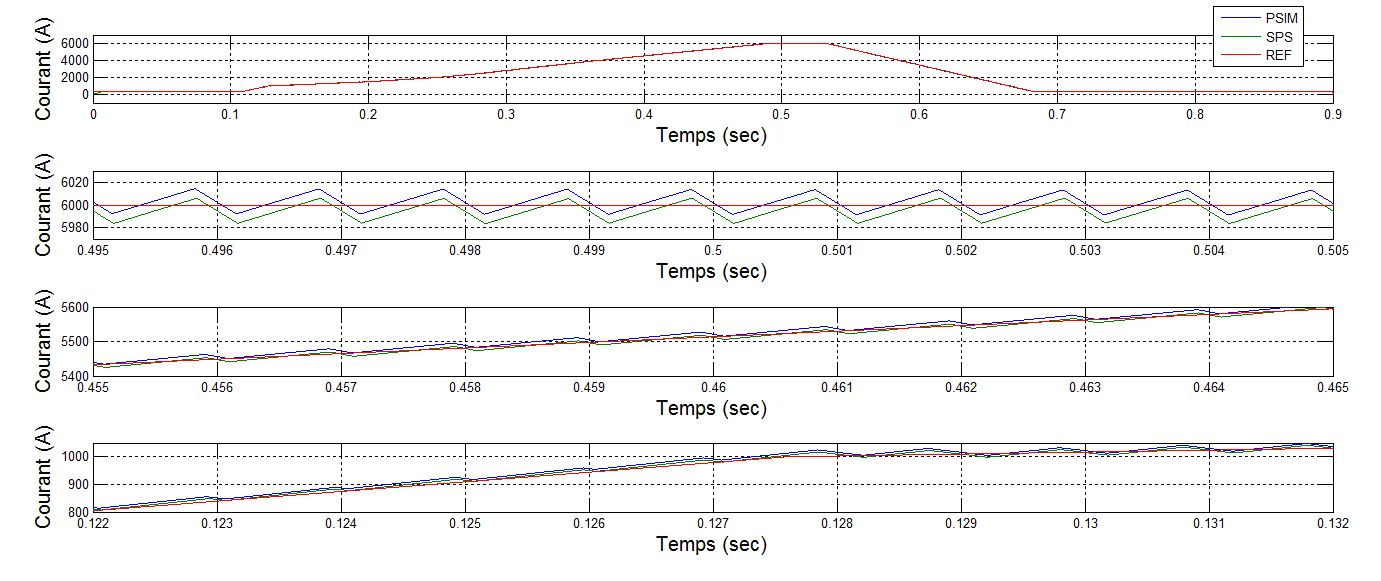
\includegraphics[scale=0.5]{Fig/Hacheur4Quadrants/HacheurCourantCharge5u.jpg}
\caption{Courant traversant la charge sur PSIM et SPS pour un pas de calcul de 5$\mu$s}
\label{hc_cou_ch_5}
\end{figure}


\begin{figure}[htb]
\centering
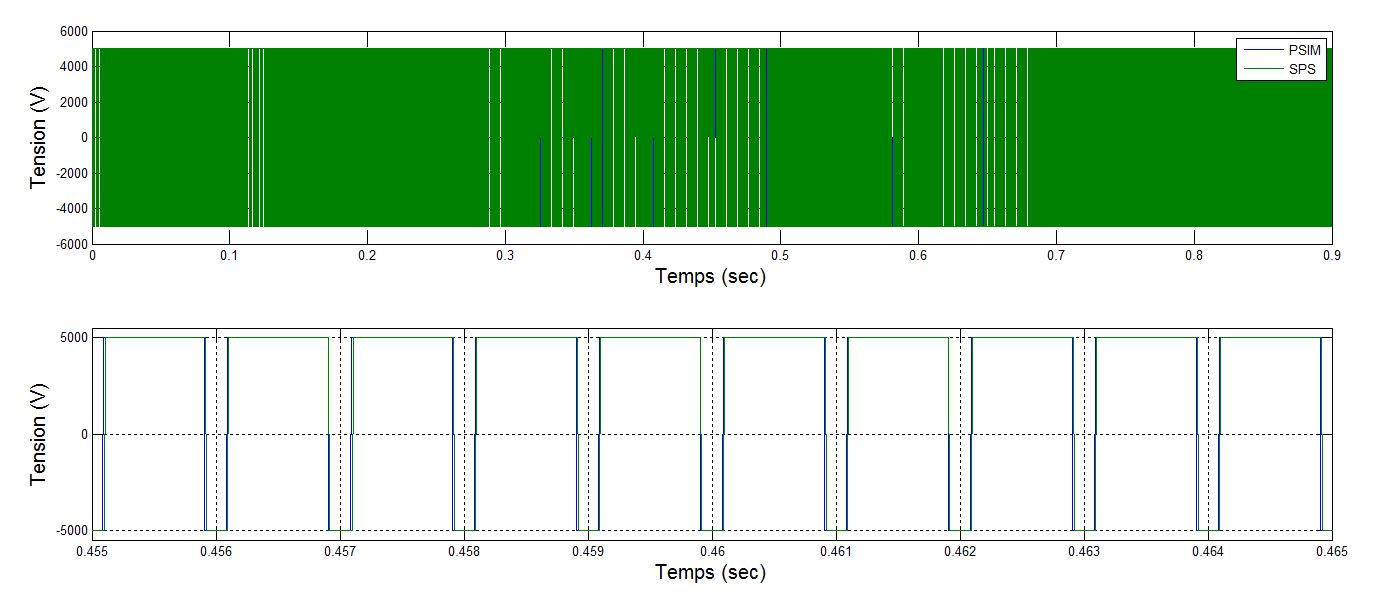
\includegraphics[scale=0.5]{Fig/Hacheur4Quadrants/HacheurTensionCharge5u.jpg}
\caption{Tension aux bornes de la charge sur PSIM et SPS pour un pas de calcul de 5$\mu$s}
\label{hc_ten_ch_5}
\end{figure}


\begin{figure}[htb]
\centering
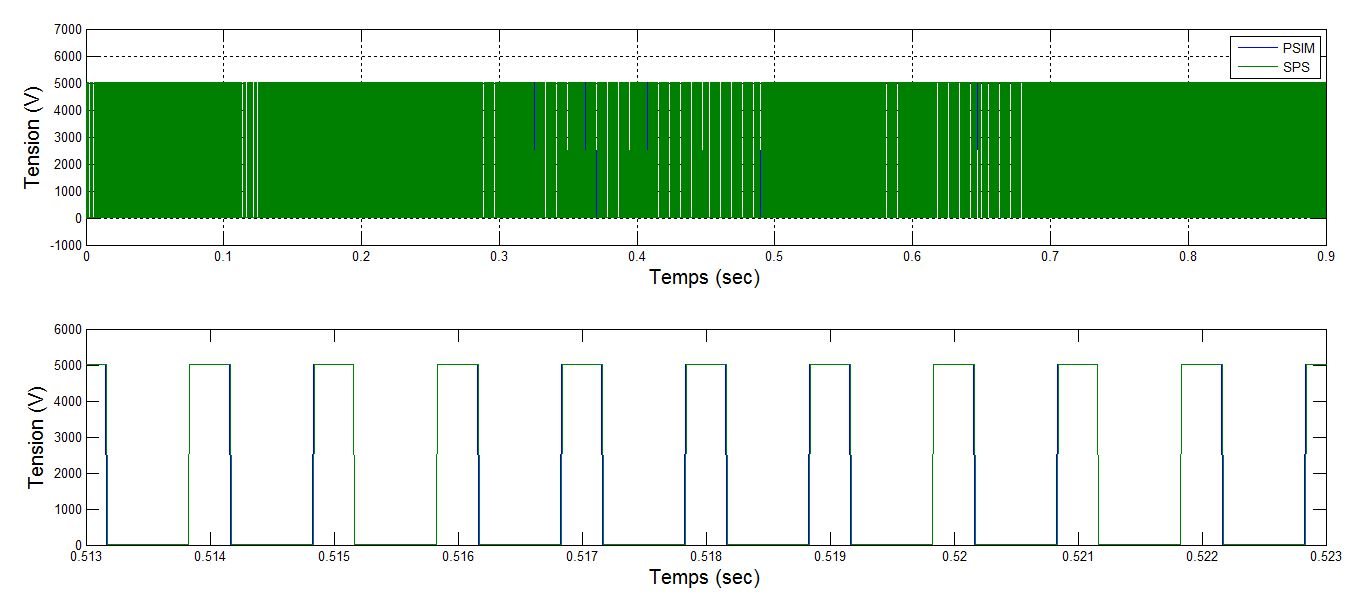
\includegraphics[scale=0.5]{Fig/Hacheur4Quadrants/HacheurTensionIGBT5u.jpg}
\caption{Tension aux bornes d'un IGBT sur PSIM et SPS pour un pas de calcul de 5$\mu$s}
\label{hc_IG_ten_5}
\end{figure}

\clearpage
\subsubsection{Vérification pour un pas de calcul de 1$\mu$s}
Cette section présente les courbes d'intérêt pour un pas de calcul discret de 1$\mu$s.


\begin{figure}[htb]
\centering
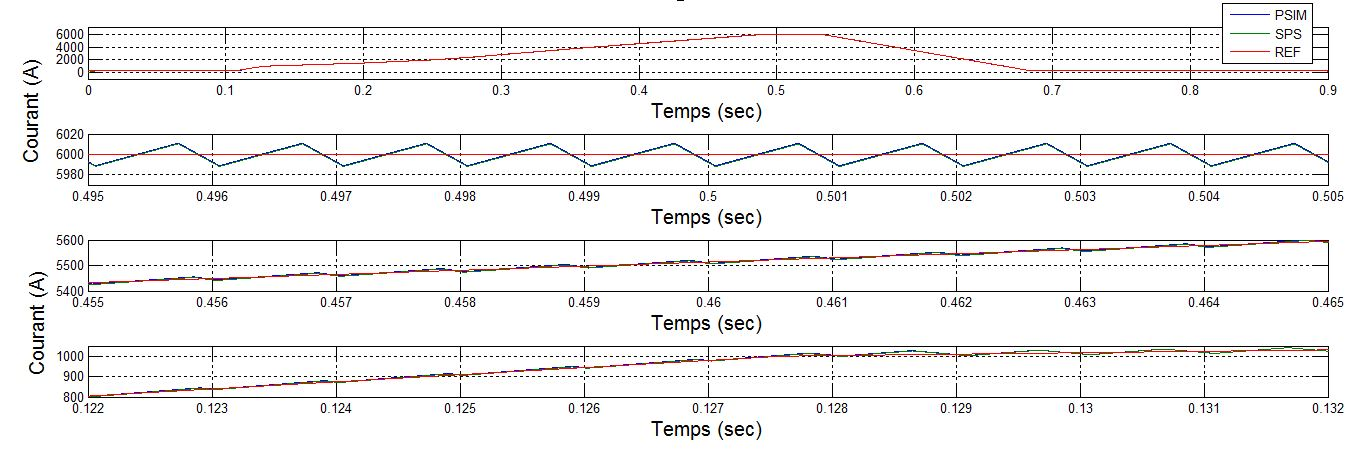
\includegraphics[scale=0.5]{Fig/Hacheur4Quadrants/HacheurCourantCharge1u.jpg}
\caption{Courant traversant la charge sur PSIM et SPS pour un pas de calcul de 1$\mu$s}
\label{hc_cou_ch_1}
\end{figure}


\begin{figure}[htb]
\centering
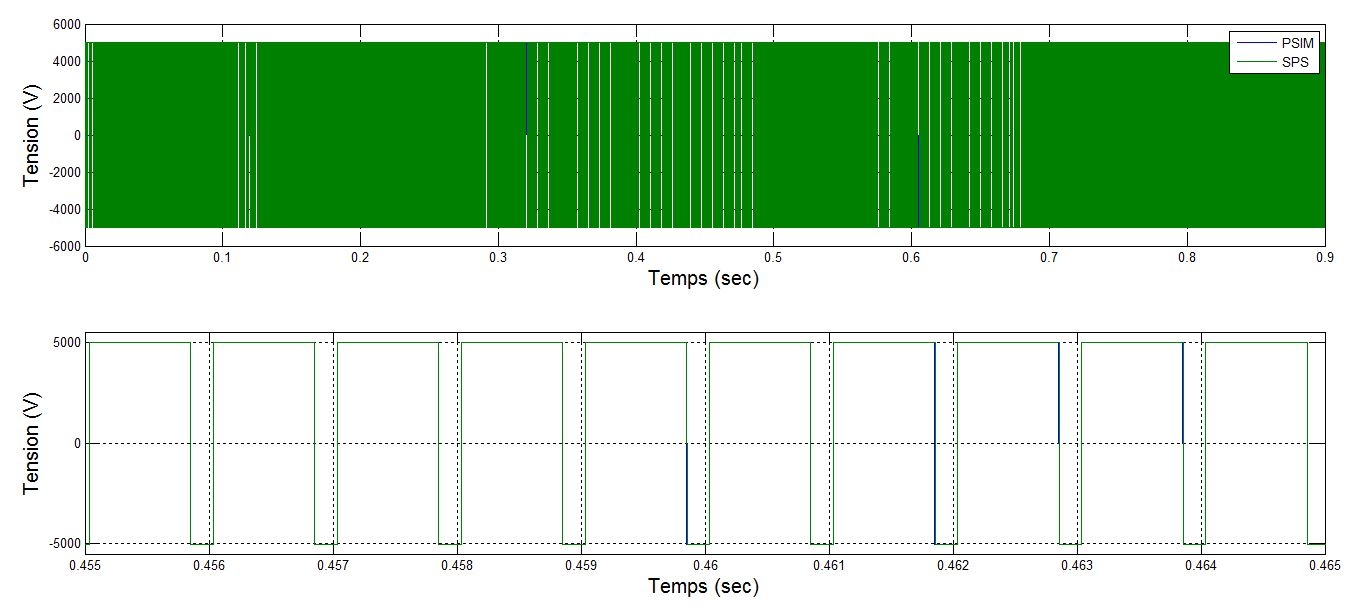
\includegraphics[scale=0.5]{Fig/Hacheur4Quadrants/HacheurTensionCharge1u.jpg}
\caption{Tension aux bornes de la charge sur PSIM et SPS pour un pas de calcul de 1$\mu$s}
\label{hc_ten_ch_1}
\end{figure}


\begin{figure}[htb]
\centering
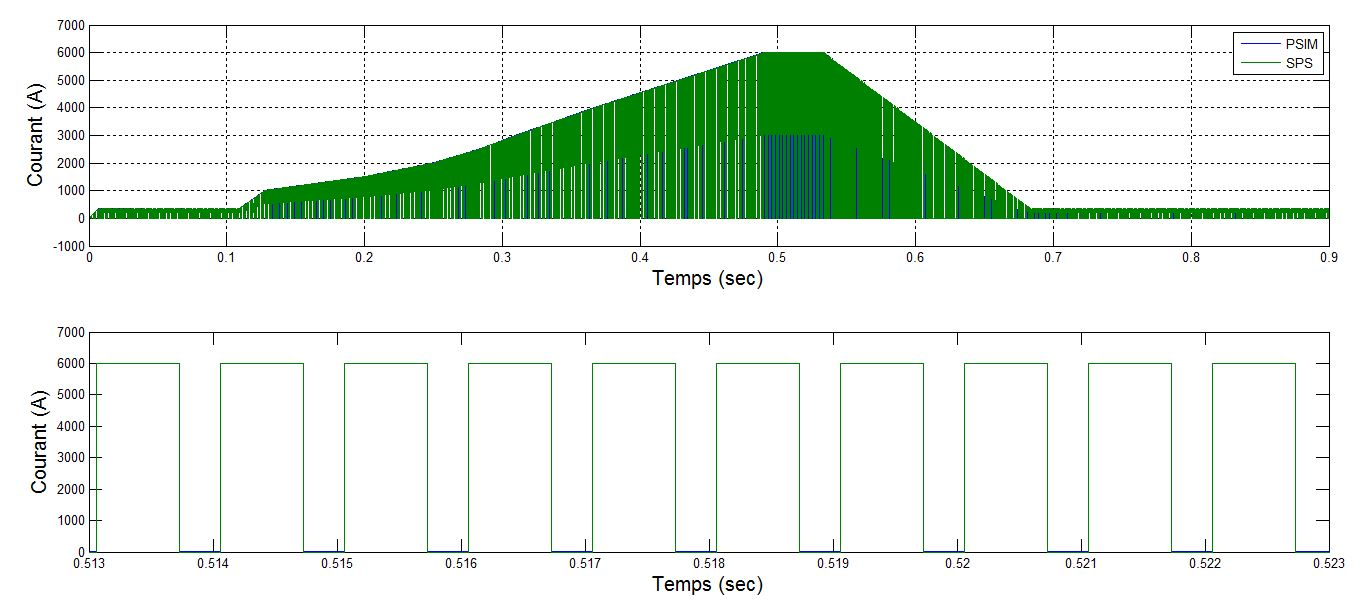
\includegraphics[scale=0.5]{Fig/Hacheur4Quadrants/HacheurCourantIGBT1u.jpg}
\caption{Courant traversant un IGBT sur PSIM et SPS pour un pas de calcul de 1$\mu$s}
\label{hc_IG_cou_1}
\end{figure}

\begin{figure}[htb]
\centering
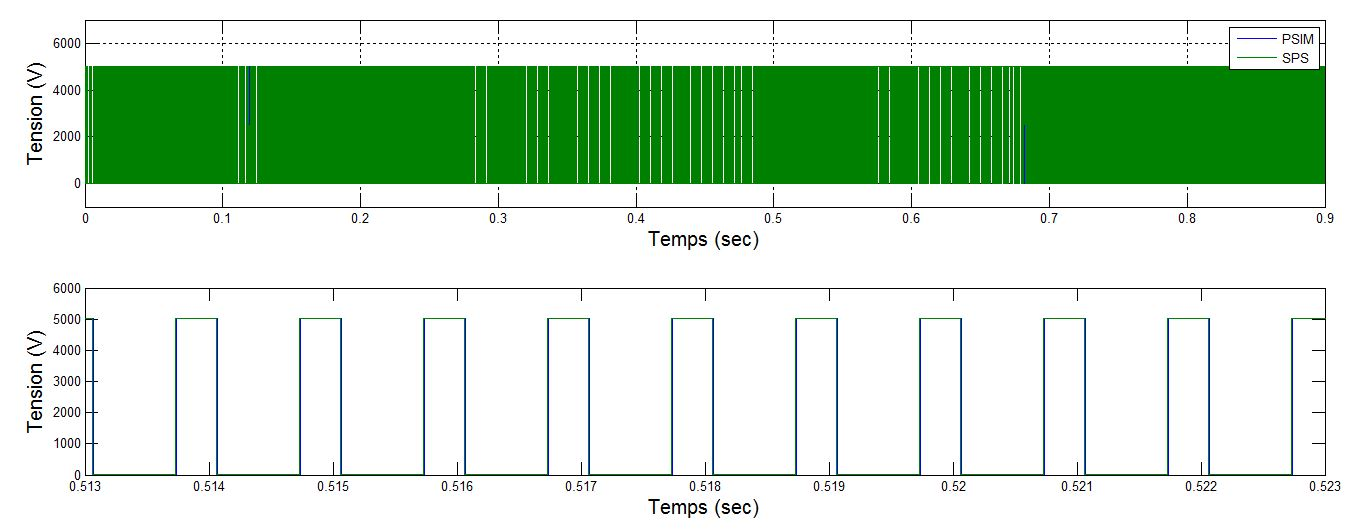
\includegraphics[scale=0.5]{Fig/Hacheur4Quadrants/HacheurTensionIGBT1u.jpg}
\caption{Tension aux bornes d'un IGBT sur PSIM et SPS pour un pas de calcul de 1$\mu$s}
\label{hc_IG_ten_1}
\end{figure}


\clearpage

\subsection{DCP/DCN}

\subsubsection{Vérification à un pas de calcul de 50$\mu$s}
Cette section présente les courbes d'intérêt pour un pas de calcul discret de 50$\mu$s.


\begin{figure}[htb]
\centering
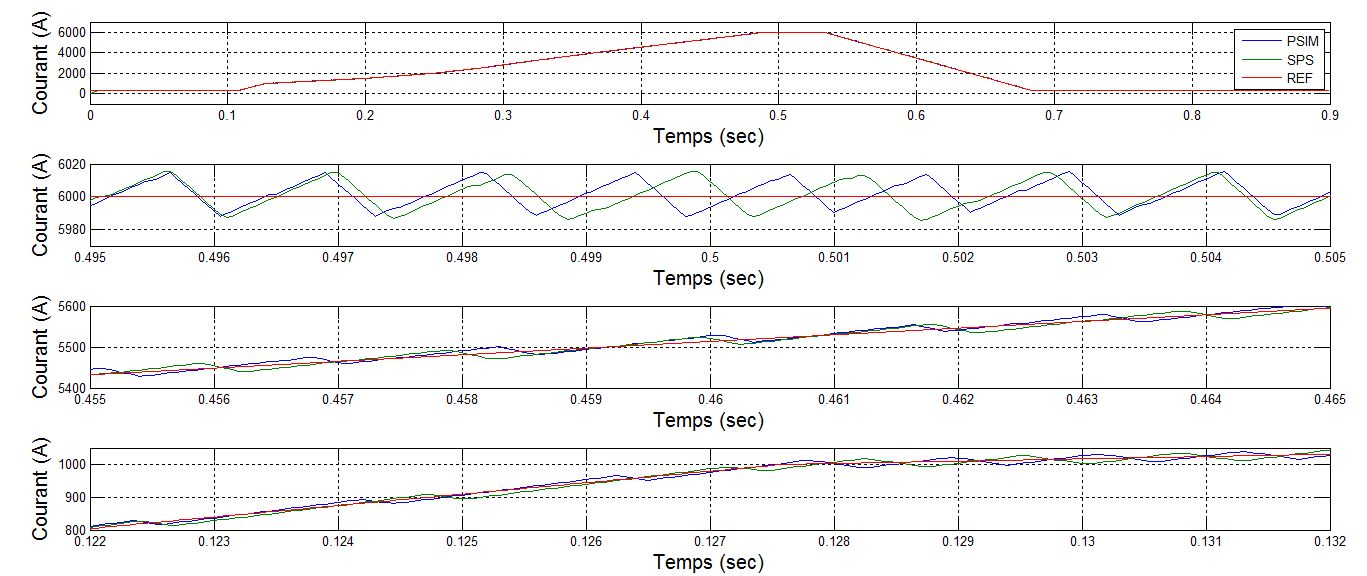
\includegraphics[scale=0.5]{Fig/DCPDCN/DCPCourantCharge50u.jpg}
\caption{Courant traversant la charge sur PSIM et SPS pour un pas de calcul de 50$\mu$s}
\label{DC_ch_cou_50}
\end{figure}


\begin{figure}[htb]
\centering
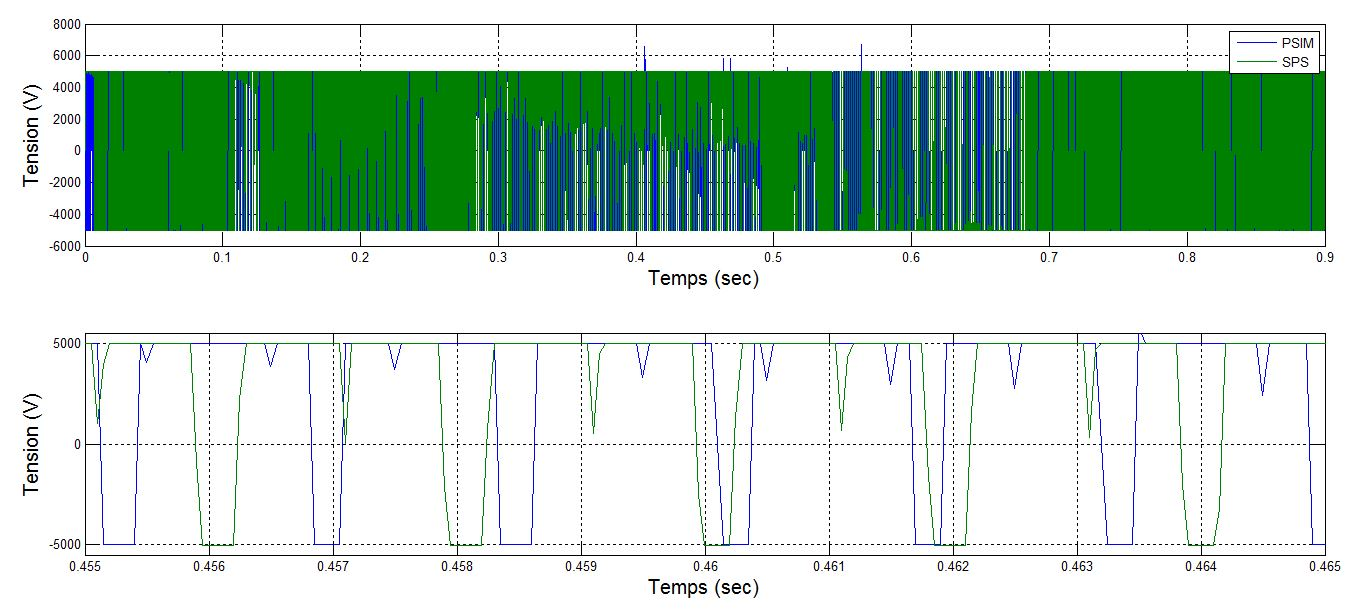
\includegraphics[scale=0.5]{Fig/DCPDCN/DCPTensionCharge50u.jpg}
\caption{Tension aux bornes de la charge sur PSIM et SPS pour un pas de calcul de 50$\mu$s}.
\label{DC_ch_ten_50}
\end{figure}

\begin{figure}[htb]
\centering
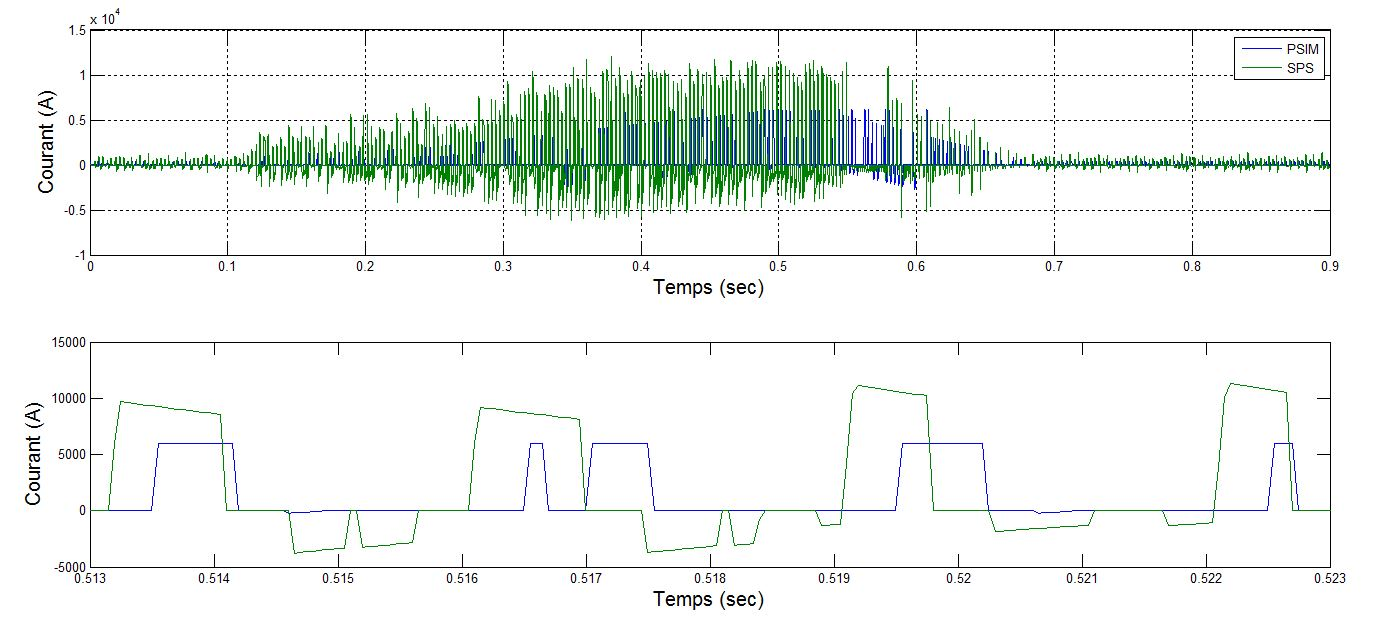
\includegraphics[scale=0.5]{Fig/DCPDCN/DCPCourantIGBT50u.jpg}
\caption{Courant traversant un IGBT sur PSIM et SPS pour un pas de calcul de 50$\mu$s}
\label{DC_IG_cou_50}
\end{figure}

\begin{figure}[htb]
\centering
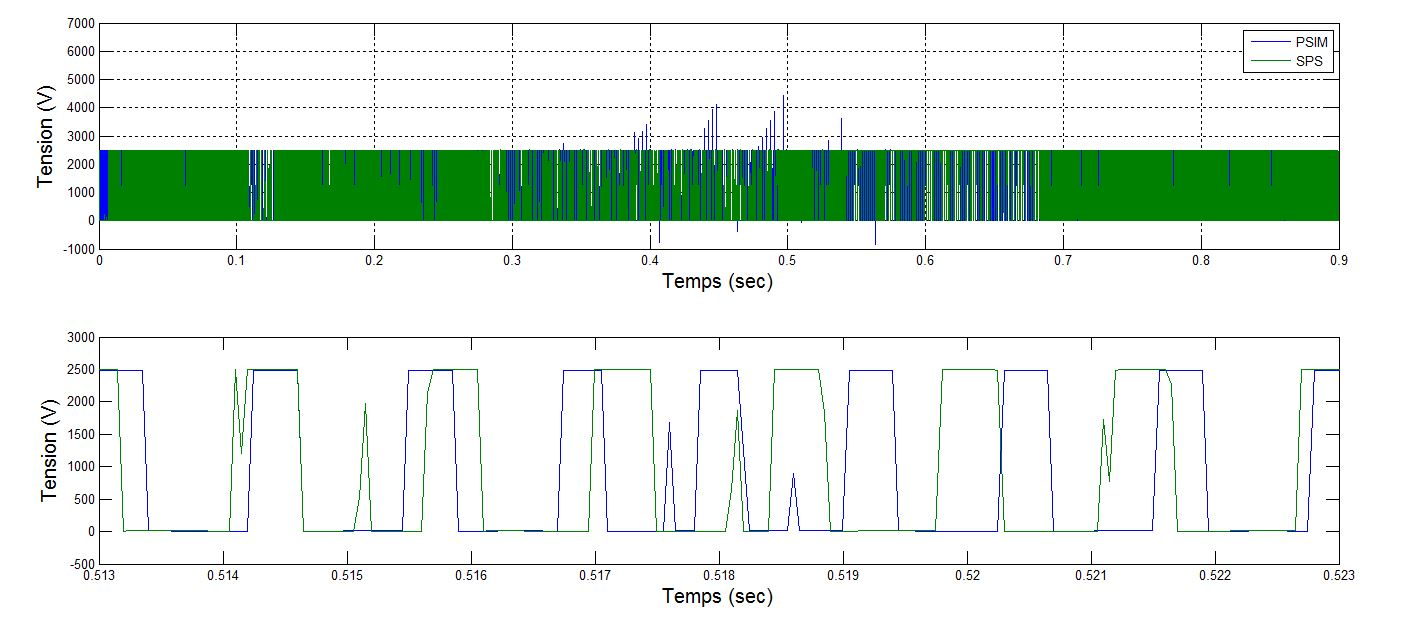
\includegraphics[scale=0.5]{Fig/DCPDCN/DCPTensionIGBT50u.jpg}
\caption{Tension au niveau d'un IGBT sur PSIM et SPS pour un pas de calcul de 50$\mu$s}
\label{DC_IG_ten_50}
\end{figure}


\clearpage

\subsubsection{Vérification à pas de calcul de 5$\mu$s}
Cette section présente les courbes d'intérêt pour un pas de calcul discret de 5$\mu$s.

\begin{figure}[htb]
\centering
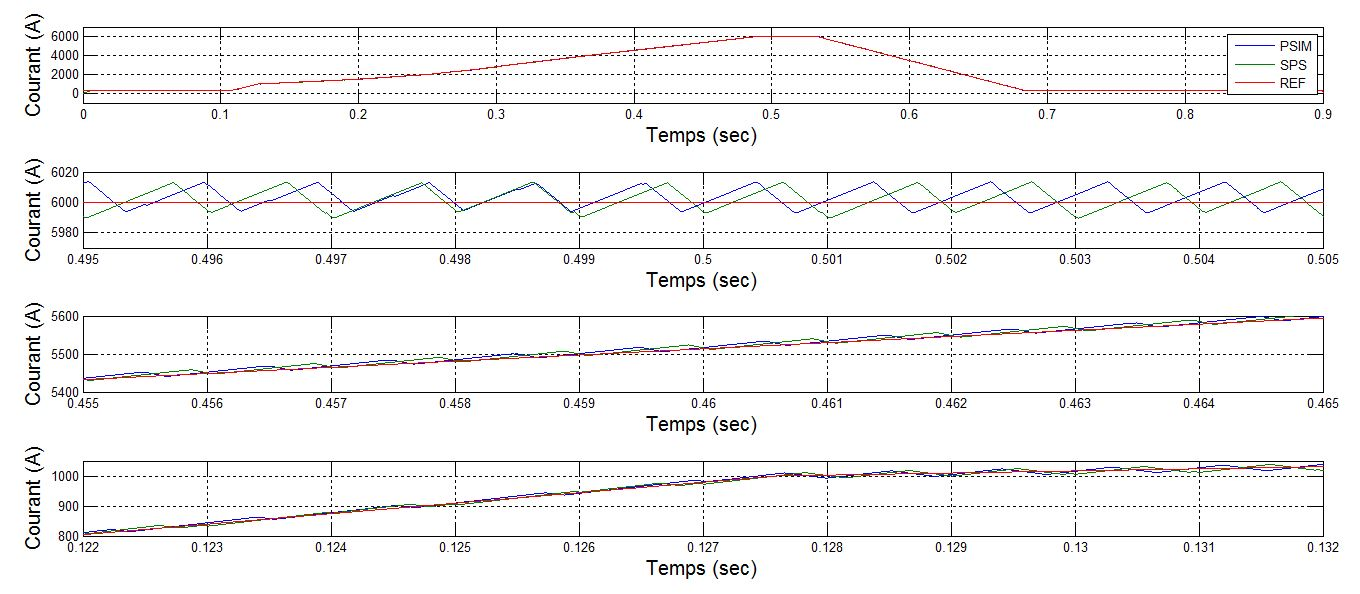
\includegraphics[scale=0.5]{Fig/DCPDCN/DCPCourantCharge5u.jpg}
\caption{Courant traversant la charge sur PSIM et SPS pour un pas de calcul de 5$\mu$s}
\label{DC_ch_cou_5}
\end{figure}


\begin{figure}[htb]
\centering
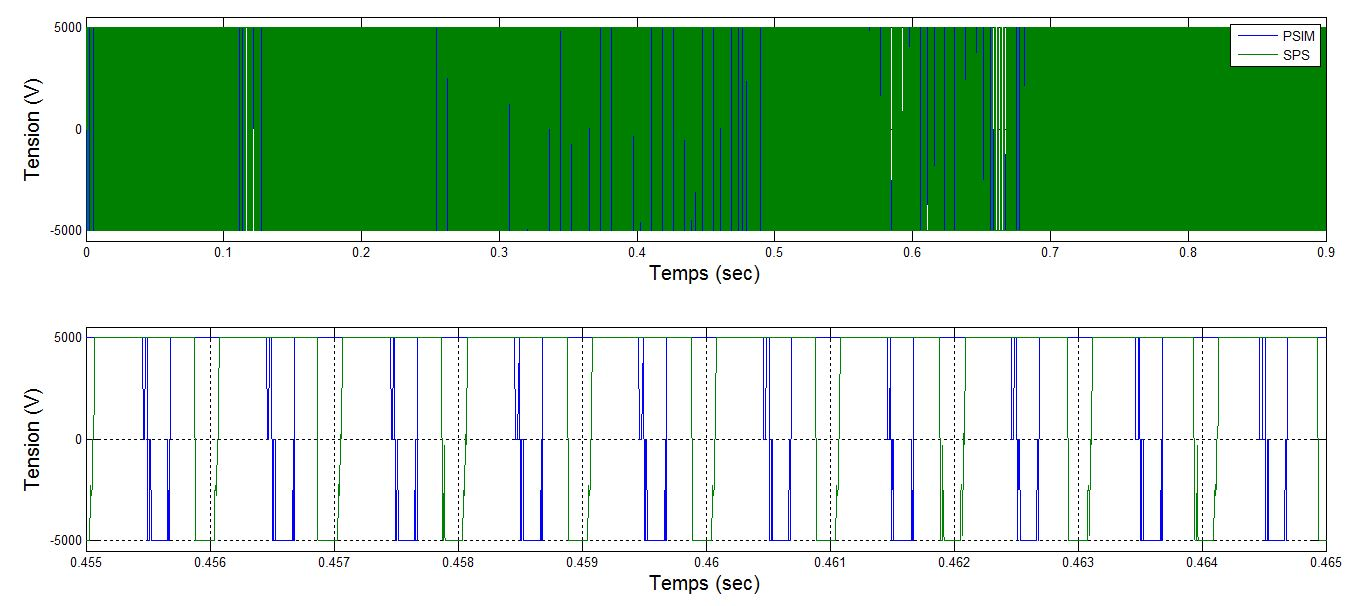
\includegraphics[scale=0.5]{Fig/DCPDCN/DCPTensionCharge5u.jpg}
\caption{Tension aux bornes de la charge sur PSIM et SPS pour un pas de calcul de 5$\mu$s}
\label{DC_ch_ten_5}
\end{figure}

\begin{figure}[htb]
\centering
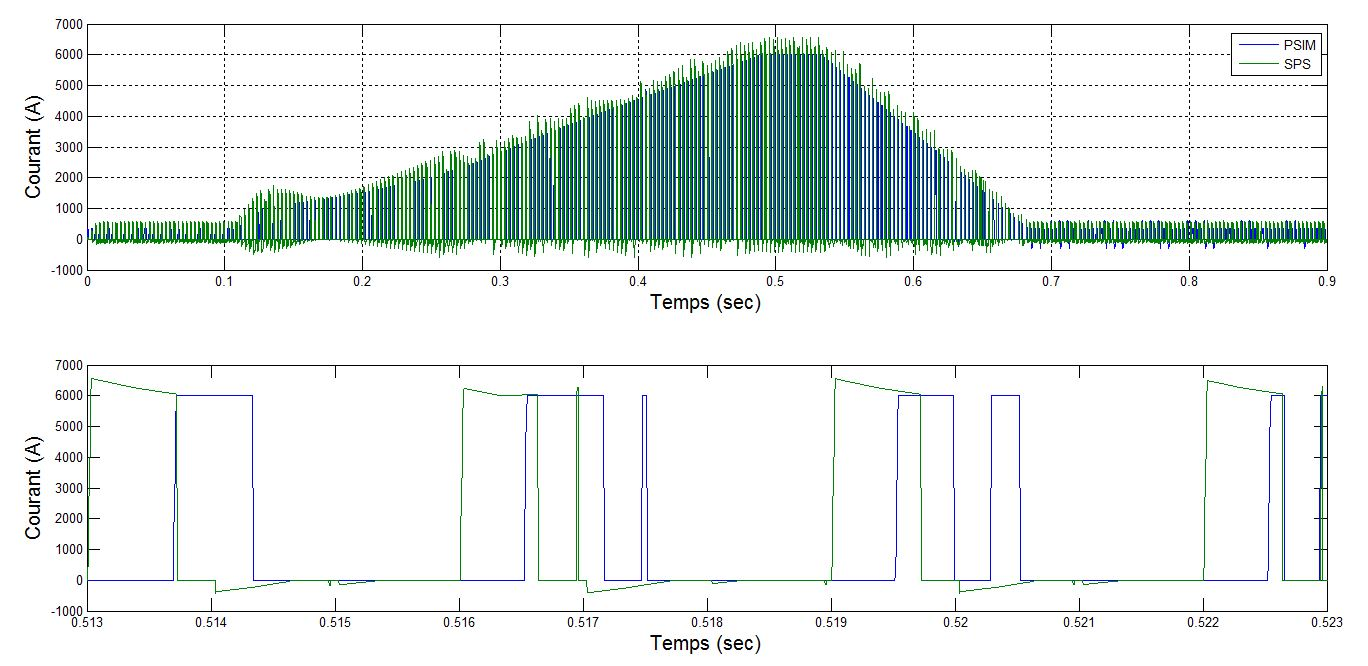
\includegraphics[scale=0.5]{Fig/DCPDCN/DCPCourantIGBT5u.jpg}
\caption{Courant traversant un IGBT sur PSIM et SPS pour un pas de calcul de 5$\mu$s}
\label{DC_IG_cou_5}
\end{figure}



\begin{figure}[htb]
\centering
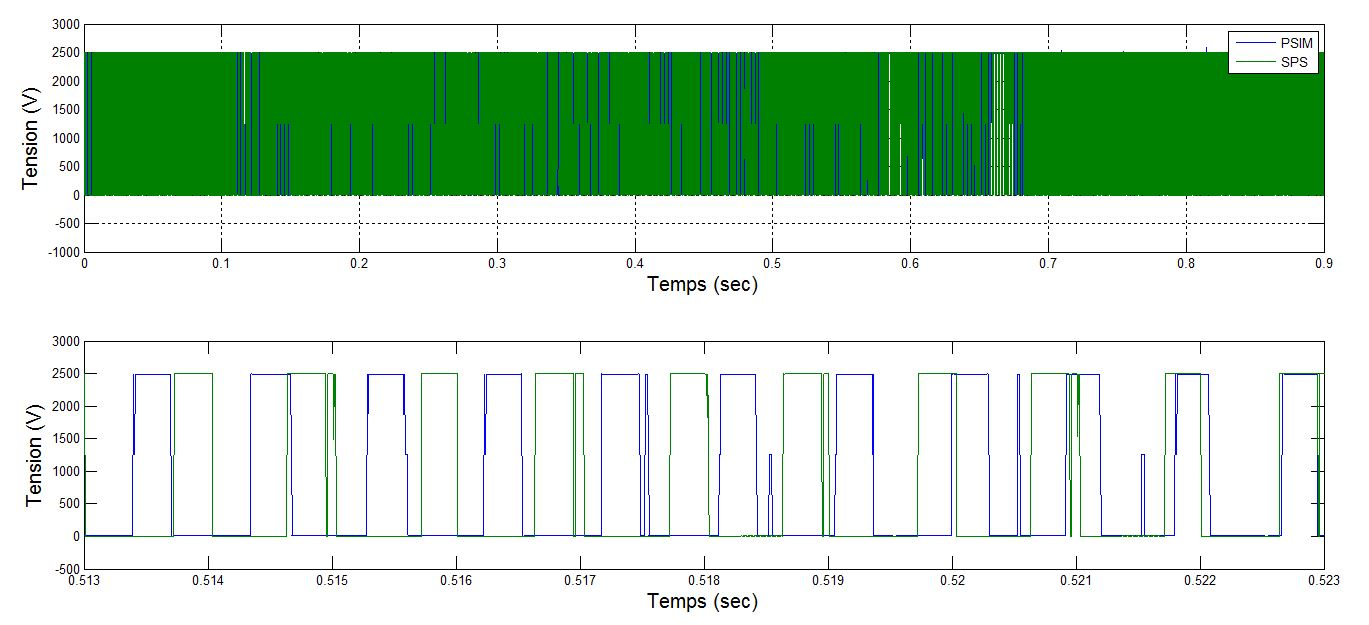
\includegraphics[scale=0.5]{Fig/DCPDCN/DCPTensionIGBT5u.jpg}
\caption{Tension traversant un IGBT sur PSIM et SPS pour un pas de calcul de 5$\mu$s}
\label{DC_IG_ten_5}
\end{figure}



\clearpage
\subsubsection{Vérification à un pas de calcul de 1us}
Cette section présente les courbes d'intérêt pour un pas de calcul discret de 1$\mu$s.


\begin{figure}[htb]
\centering
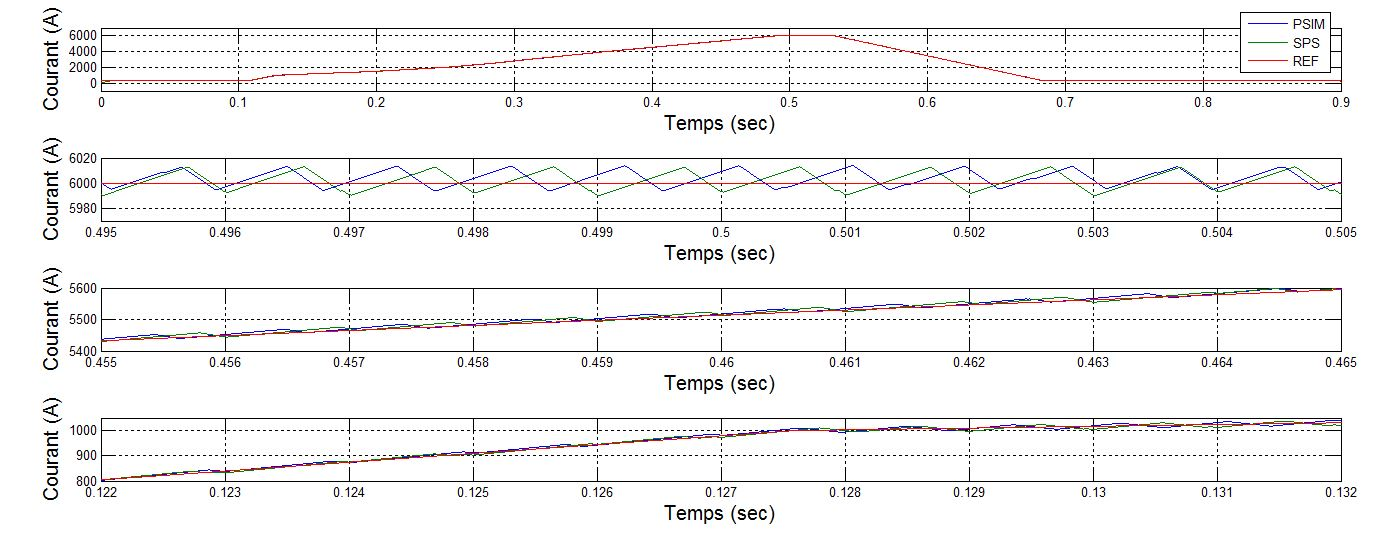
\includegraphics[scale=0.5]{Fig/DCPDCN/DCPCourantCharge1u.jpg}
\caption{Courant traversant la charge sur PSIM et SPS pour un pas de calcul de 1$\mu$s}
\label{DC_ch_cou_1}
\end{figure}


\begin{figure}[htb]
\centering
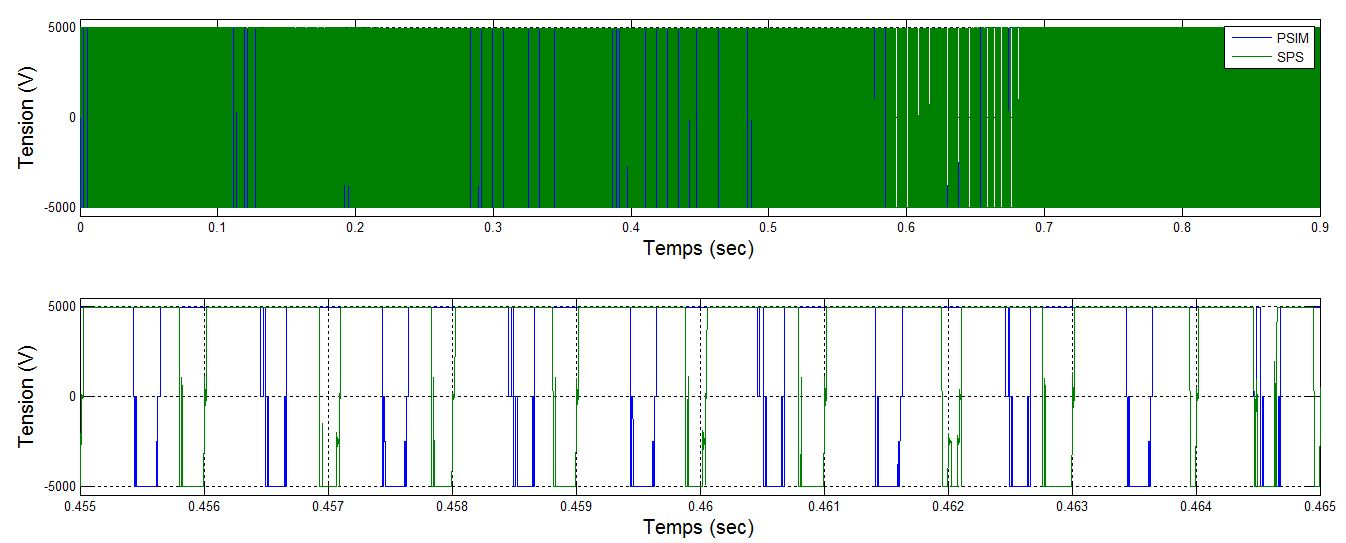
\includegraphics[scale=0.5]{Fig/DCPDCN/DCPTensionCharge1u.jpg}
\caption{Tension aux bornes de la charge sur PSIM et SPS pour un pas de calcul de 1$\mu$s}
\label{DC_ch_ten_1}
\end{figure}


\begin{figure}[htb]
\centering
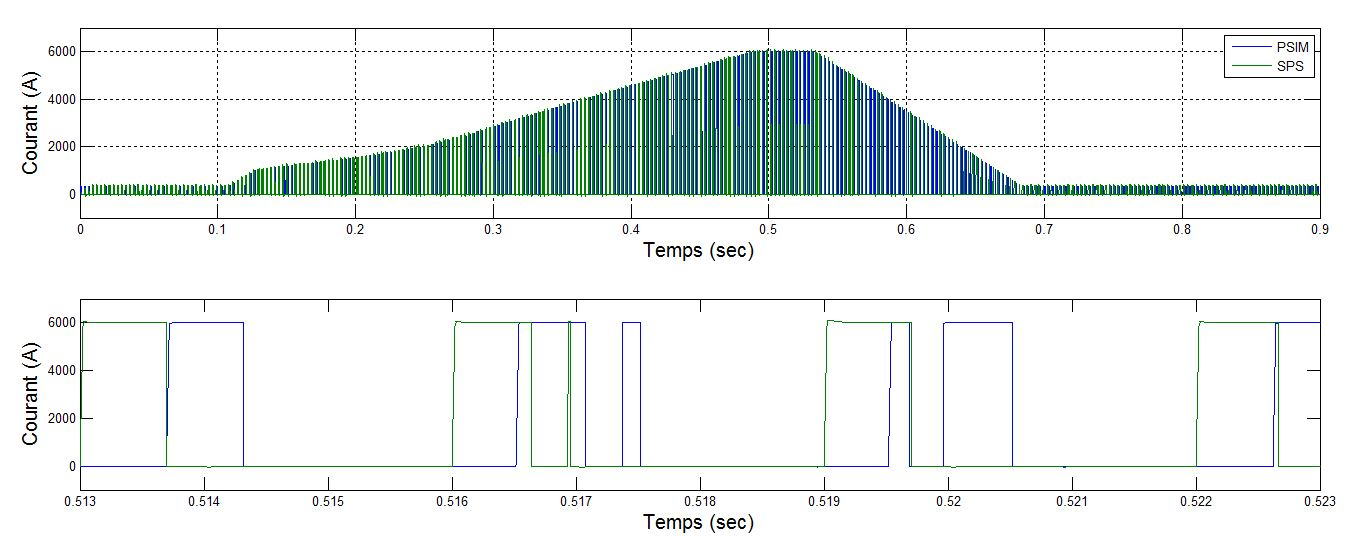
\includegraphics[scale=0.5]{Fig/DCPDCN/DCPCourantIGBT1u.jpg}
\caption{Courant traversant un IGBT sur PSIM et SPS pour un pas de calcul de 1$\mu$s}
\label{DC_IG_cou_1}
\end{figure}


\begin{figure}[htb]
\centering
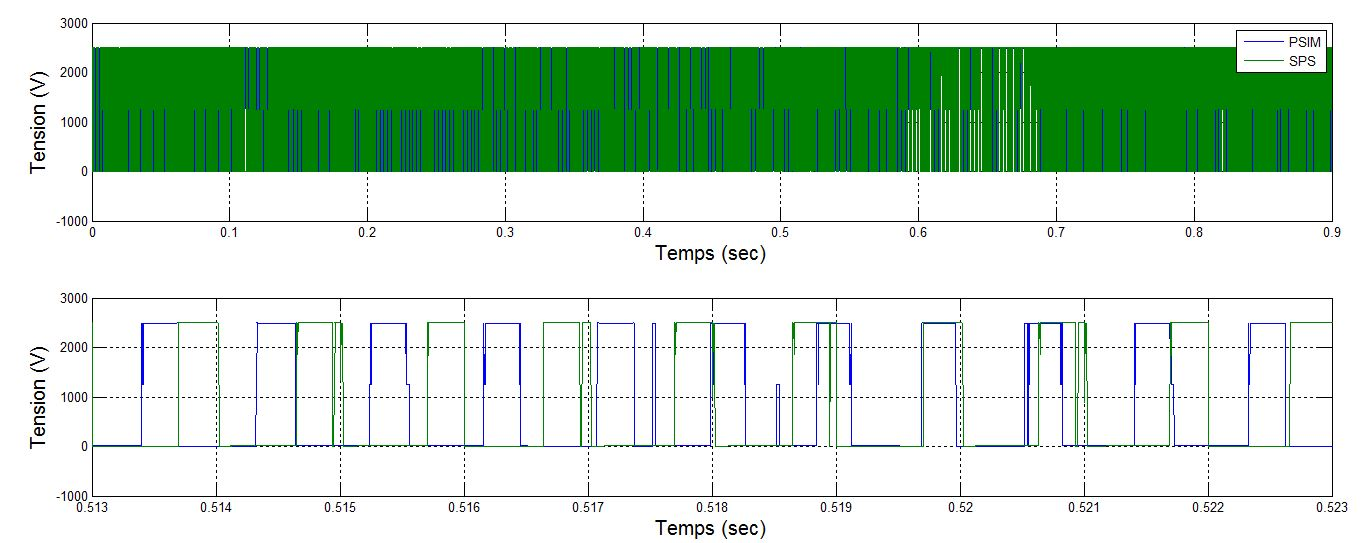
\includegraphics[scale=0.5]{Fig/DCPDCN/DCPTensionIGBT1u.jpg}
\caption{Tension aux bornes d'un IGBT sur PSIM et SPS pour un pas de calcul de 1$\mu$s}
\label{DC_IG_ten_1}
\end{figure}






\end{document}